\documentclass[12pt]{article}
\setlength\parindent{0pt}
\usepackage{fullpage}
\usepackage{amsmath}
\usepackage{graphicx}
\usepackage{color}
\definecolor{Red}           {rgb}{1,0.3,0.0}
\setlength{\parskip}{4mm}
\def\LL{\left\langle}   % left angle bracket
\def\RR{\right\rangle}  % right angle bracket
\def\LP{\left(}         % left parenthesis
\def\RP{\right)}        % right parenthesis
\def\LB{\left\{}        % left curly bracket
\def\RB{\right\}}       % right curly bracket
\def\PAR#1#2{ {{\partial #1}\over{\partial #2}} }
\def\PARTWO#1#2{ {{\partial^2 #1}\over{\partial #2}^2} }
\def\PARTWOMIX#1#2#3{ {{\partial^2 #1}\over{\partial #2 \partial #3}} }
\newcommand{\BI}{\begin{itemize}}
\newcommand{\EI}{\end{itemize}}
\newcommand{\BE}{\begin{displaymath}}
\newcommand{\EE}{\end{displaymath}}
\newcommand{\BNE}{\begin{equation}}
\newcommand{\ENE}{\end{equation}}
\newcommand{\BEA}{\begin{eqnarray}}
\newcommand{\EEA}{\nonumber\end{eqnarray}}
\newcommand{\EL}{\nonumber\\}
\newcommand{\la}[1]{\label{#1}}
\newcommand{\ie}{{\em i.e.\ }}
\newcommand{\eg}{{\em e.\,g.\ }}
\newcommand{\cf}{cf.\ }
\newcommand{\etc}{etc.\ }
\newcommand{\Tr}{{\rm tr}}
\newcommand{\etal}{{\it et al.}}
\newcommand{\OL}[1]{\overline{#1}\ } % overline
\newcommand{\OLL}[1]{\overline{\overline{#1}}\ } % double overline
\newcommand{\OON}{\frac{1}{N}} % "one over N"
\newcommand{\OOX}[1]{\frac{1}{#1}} % "one over X"



\begin{document}
\pagenumbering{gobble}
\Large
\centerline{\sc{Recitation Exercises}}
\normalsize
\centerline{\sc{Week 6, Day 1}}

\medskip
\centerline{\Large Question 1: Practice from Earlier (this should be quick)}

\begin{minipage}{0.5\textwidth}
	Consider a ball tethered to a rotating pole by two cables of equal length as shown to the right. The ball rotates along with the pole, making a horizontal circle (shown in green on the diagram). Suppose that you know the ball has a mass $m$, the pole is rotating at angular velocity $\omega$, and the radius of the circle it makes is $r$.
	
	\bigskip
	
	You want to find the relationship between $m$, $\omega$, $r$, and the tensions in the cables $T_1$ and $T_2$.
	
\end{minipage}
\begin{minipage}{0.4\textwidth}
	\hspace{0.1\textwidth}
	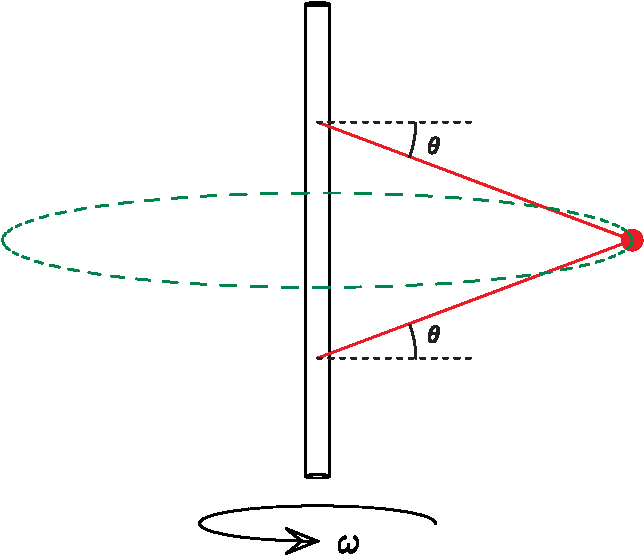
\includegraphics[width=0.9\textwidth]{pole-crop.pdf}
\end{minipage}

Draw a force diagram for the ball below, and indicate your choice of coordinate system.
%
%{\color{Red} This is just for practice in case anyone gets done or wants extra practice. This is a former exam problem.}

\vspace{3in}

Construct Newton's laws in both $x$ and $y$ for the ball based on your force diagram, putting in what you know about $a_x$ and $a_y$. (You don't need to actually solve the system of equations, but show it to your TA/coach.)
%
%{\color{Red}
%
%\begin{align*}
%T_1 \cos \theta + T_2 \cos \theta\hspace{2.6em} &= m \omega^2 r \\
%T_1 \sin \theta - T_2 \sin \theta - mg &= 0
%\end{align*}
%
%They shouldn't feel the need to go any further than this.


\newpage

\centerline{\Large Question 2: variation of apparent weight with latitude}

\medskip

{\footnotesize Note about this exercise: This question asks you to consider what $g$ means, and how it might vary on Earth's surface. The effect you are studying here is the reduction in apparent weight because of the Earth's rotation. There are smaller effects from the ``non-roundness'' of the Earth which we don't care about here. Ultimately this means that the apparent weight of a 1 kg mass is around 9.83 N at the North (or South) Pole and 9.78 N at the Equator. It is 9.81 N only in latitudes corresponding to Paris, Berlin, or Kyiv; in New York it is closer to 9.80 N, and in the tropical latitudes where many people live (most of Africa, South Asia, most of South America) it is 9.79 N or 9.78 N, to three significant digits. This means that insisting on $g=9.81\,\rm m/\rm s^2$ isn't correct for most of us (unless you are in Europe or Canada).
}


\it For this problem, do all calculations to five significant digits. Some figures that will be useful:

\rm
\BI
\item Mass of Earth: $5.9722\times 10^{24}$ kg
\item Radius of Earth: $ 6.3710 \times 10^6$ m (assume it is spherical; we don't have the math to deal with its oblateness)
\item Gravitational constant (G): $6.6741 \times 10^{-11} \,\rm N\cdot \rm m^2/{\rm kg}^2$
\item Length of one day: $8.6400 \times 10^4$ s
\EI


a) Using Newton's law of universal gravitation $F_g=\frac{GMm}{r^2}$, determine the force of gravity on a 1 kg mass resting on the surface of the Earth. Are you surprised by this figure?
%
%{\color{Red} This gives 9.82001 N for the force of gravity on a thing on Earth's surface. This is the same everywhere -- remember we are not thinking about Earth's oblateness here. 
%	It may be a surprise to people who were expecting a clean 9.81... Here the students might try to make things harder than they need to be -- here we want them to do the simplest possible thing.
%}
\vspace{2in}

b) Suppose this mass were resting on a scale sitting on the North Pole owned by Santa Claus. Recall that scales measure
the normal force that they exert. What value would Santa's scale read? What would Santa conclude the value of $g$ is?
%
%{\color{Red} The students might overcomplicate this. Since the things are just sitting on Earth's surface, for this and everything else, $F_N - F_g = ma$. Here $a=0$. But they can't use $F_g = mg$, since we don't know what ``g" is. Since $a=0$ the normal force is just 9.82001 N again.
%
%The students should not spend too much time here.
%}

\newpage

c) Suppose that an identical 1 kg mass were resting on a scale sitting on the Equator, somewhere in Kenya. What would {\it this} scale read? (Hint: What is the acceleration of the mass?) What would our Kenyan physicist conclude about $g$?
%
%{\color{Red} Here is where the substance is. The realization that we are all accelerating (except Santa) is critical here. We are not used to thinking that way! Remember that the acceleration is {\it inward}, so 
%	
%	$$F_N - F_g = -m\omega^2 r \rightarrow F_N = F_g - m \omega^2 r.$$
%	
%	This is the critical result -- that your apparent weight goes down when you stand on the Equator. The normal force is 9.78628 N.
%}

\vspace{3in}

d) This problem shows that your apparent weight depends on your location on Earth. 
Does it make sense to define $g$ as $F_g/m$ 
(the strength of the gravitational force divided by an object's mass) or
$F_N/m$ (the strength of the normal force, and thus the scale reading, divided by mass)? Call your TA/coach over to join your conversation.

\vspace{1in}

%{\color{Red}
%	
%	Either result makes sense, of course -- it's all a matter of definition. However, using the value of $g$ coming only from the Earth's gravitational force means that we will constantly need to think about the acceleration of Earth's surface. But using $g = F_N/m$, which gives the acceleration of things in freefall {\it minus the acceleration of Earth's surface} allows us to treat objects sitting on Earth's surface as not accelerating.
%}


e) Is this distinction likely to be relevant to the sort of engineering or science you will do during your
career? (The answer will depend on what you will do, of course!)


%\newpage
%
%\centerline{\Large Question 4: universal gravitation and the Sun's mass}
%
%In this problem, you will compute the mass of the Sun. The Earth’s orbit is very nearly circular,
%and the earth is 150 million km from the Sun.
%
%a) What is the angular velocity of the Earth in its orbit?
%
%\vspace{2in}
%
%b) What is the tangential velocity of the Earth? 
%
%\vspace{1in}
%
%c) What is the radial acceleration of the Earth?
%
%\vspace{1in}
%
%d) What is the mass of the Sun?
%
%\newpage
%
\newpage
\centerline{\Large Question 3: Weightlessness}

Astronauts in orbit around the Earth are not ``so far away that they don't feel Earth's gravity'';
actually, they’re quite close to the surface. However, we’ve all seen the videos of astronauts drifting
around ``weightlessly'' in the International Space Station.

a) Explain how an astronaut can be under the influence of Earth's gravity, and yet exert no normal
force on the surface of the spacecraft they are standing in.
%
%{\color{Red}Normal forces stop objects from moving through other objects, and no extra normal force is required for them to not move through the surface of the spacecraft. Under the influence of Earth's gravity alone, the spacecraft accelerates downward at the same rate that they do, so the floor doesn't have to push on them.}

\vspace{2in}

b) Draw a force diagram for the astronaut floating in the middle of the Space Station, not touching
any of the walls or floor. How do you reconcile your diagram with the fact that the astronaut
doesn't seem to fall?
%
%{\color{Red} The diagram just has gravity pointing downward. They {\it are} falling -- so is the spacecraft around them. They aren't falling {\it into the Earth} because their horizontal / tangential velocity is fast enough that they go in a circle around it. That horizontal velocity is chosen specifically to match their altitude, such that $v^2/r = g$.}
%
\vspace{2in}

c) Is this astronaut truly ``weightless''? What does ``weightless'' mean? (There are multiple correct answers to both of these questions.)
%
%{\color{Red} If you define ``weight'' as the force of gravity, then no -- they are not weightless, since Earth's gravity still acts on them and causes them to accelerate downward. If you define ``weight'' as the magnitude of the normal force pressing on your feet, and ``weightless'' as the absence of such a force (the thing that causes us to feel heavy -- think of the elevator problem in homework, then they are ``weightless'' since no normal force presses on their feet. 
%
%I prefer the definitions:
%
%\begin{itemize}
%	\item Weight: the force of gravity acting on you (not zero here)
%	\item Apparent weight: the normal force pushing on you from below (zero here)
%\end{itemize}
%
%So by my definitions, they are not weightless but ``apparent weight-less''. Note that some textbooks use ``weight'' to mean ``apparent weight''. I think this is confusing.
%
%}

\newpage


\centerline{\Large Question 4: geostationary orbit}

It is sometimes useful to place satellites in orbit so that they stay in a fixed position relative to the
Earth; that is, their orbits are synchronized with the Earth's rotation so that a satellite might stay
above the same point on Earth’s surface all the time.

What is the altitude of such an orbit? Note that it is high enough that you need to use $F_g=\frac{GMm}{r^2}$
rather than just $F_g = mg$. {\it (Are there any meaningful forces on the satellite besides Earth's gravity?)}

{\sc Hint 1:} If this orbit is synchronized with Earth's rotation, then you should be able to figure out its
angular velocity.




{\sc Hint 2:} If you do this problem as we have guided you, by waiting to substitute numbers in until the 
very end, you will arrive at an expression relating the radius $R$ of a circular orbit with the mass $M$ of the 
planet being orbited and the angular velocity $\omega$ of the orbit. This question will be on HW5, and is related
to the derivation of Kepler's third law that you will do there.
%
%{\color{Red}
%	The angular velocity is just one rotation per day: $$\frac {2\pi\,\text{rad}}{86400\,\rm s} = 7.27 \times 10^{-5} \frac{\text{rad}}{\rm s}.$$
%
%Here students will most commonly make mistakes by, again, adding stuff that isn't there. There are no normal forces. There is no $mg$ -- we are not on Earth's surface. The only force is Earth's gravity, so we have 
%
%$$
%\frac{GMm}{r^2} = m \omega^2 r
%$$
%
%Note that $r$ here is the distance to Earth's {\it center}, not its {\it surface}. The distinction here isn't huge, but in some cases it might be.
%	
%}


\end{document}
